\section{Wähle ein Sprite aus und bewege es in 4 Richtungen}
\subsection{Aufgabe}
Scratch Exercise 1: .

Das Scratch Programm wurde am MIT entwickelt, um jungen Schülern die Programmierung und die Multimedia Kommunikation beizubringen. 

Die Programmierung erfolgt durch ein visuelles System, die Kacheln oder Tiles. Diesen können Befehle zugeordnet werden und durch das zusammenlegen der Kacheln entstehen die Programme. Die Programme steuern Figuren und Objekte innerhalb des Spiels.


\subsection{Die Scratch Oberfläche}
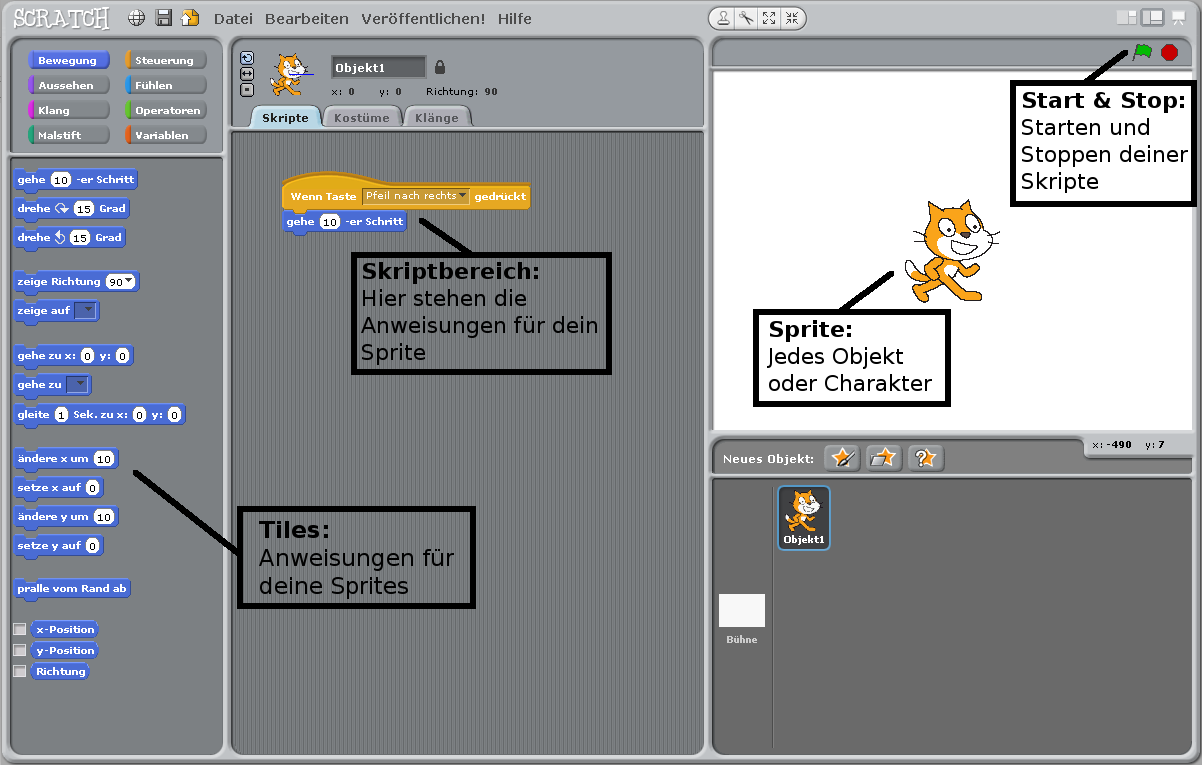
\includegraphics[width=\textwidth]{images/example1_overview.png}

\subsubsection{Wähle einen Sprite}

Ein Sprite ist eine Figur oder ein Objekt in deinem Spiel. Die Sprites können sich bewegen oder still stehen. Wir wählen eine Sprite-Figur und lassen sie über deinen Bildschirm laufen.
\begin{itemize}
\item[1.] Öffne Scratch
\item[2.] Öffne den Ordner in den Scratch installiert wurde.
\item[3.] Klicke doppelt auf das Scratch-Icon.
\item[4.] Nun siehst du den Startbildschirm.
\end{itemize}

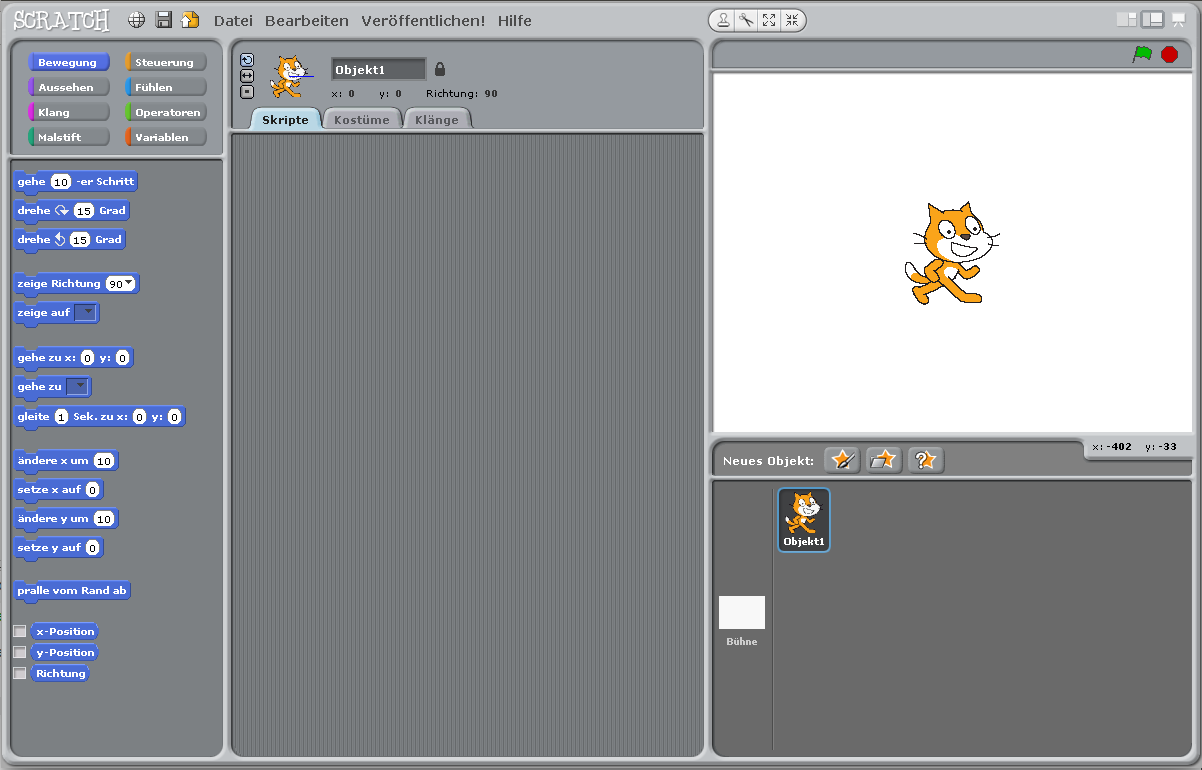
\includegraphics[width=\textwidth]{images/aufgabe1_start.png}

\begin{itemize}
\item[5.] Klicke auf den Reiter \textit{Kostüme}
\end{itemize}

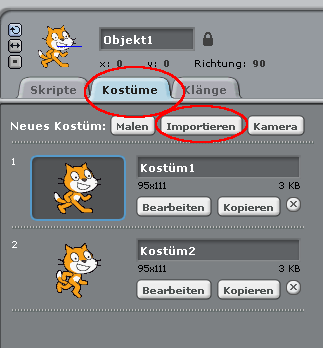
\includegraphics[width=0.5\textwidth]{images/aufgabe1_kostueme.png}

\begin{itemize}
\item[6.] Klicke auf \textit{Importieren}
\item[7.] Wähle den Ordner (Animals (dt. Tiere), People (dt. Menschen), Things (dt. Dinge)
\end{itemize}

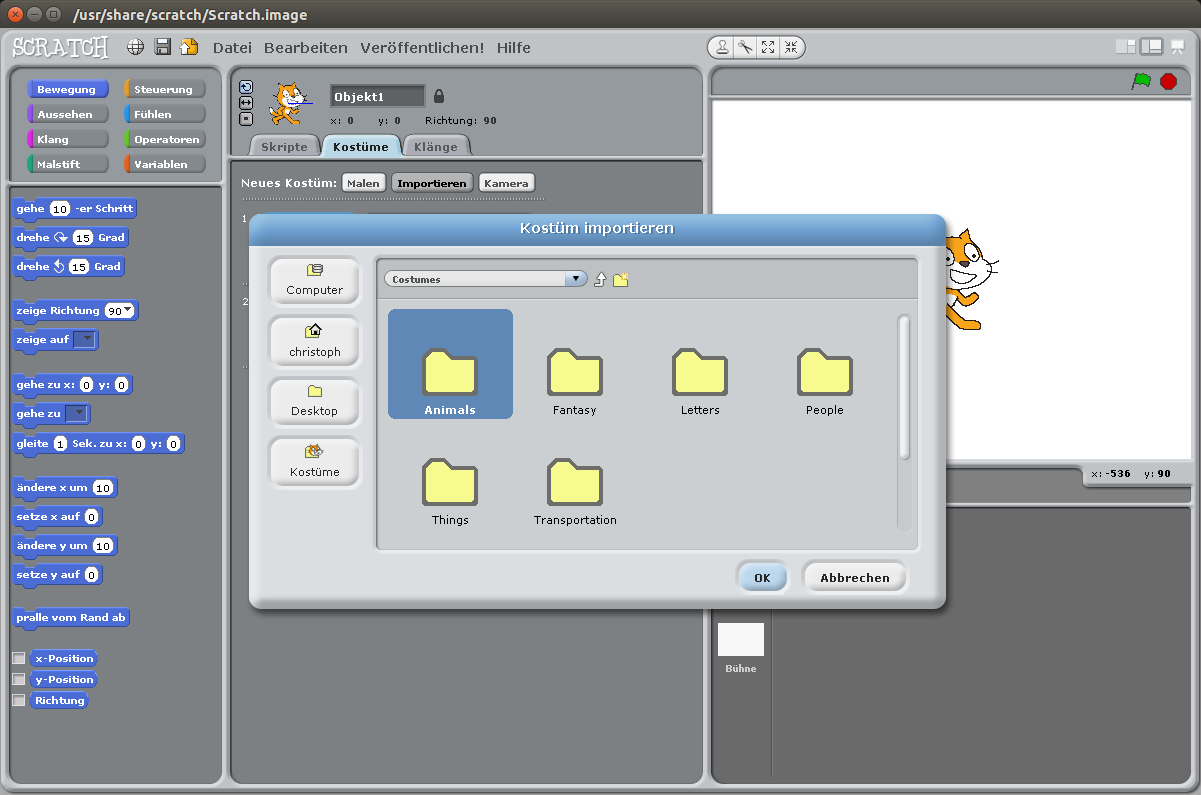
\includegraphics[width=\textwidth]{images/aufgabe1_ordner.png}

\begin{itemize}
\item[8.] Wähle einen  Sprite! (Doppelklick)
\end{itemize}

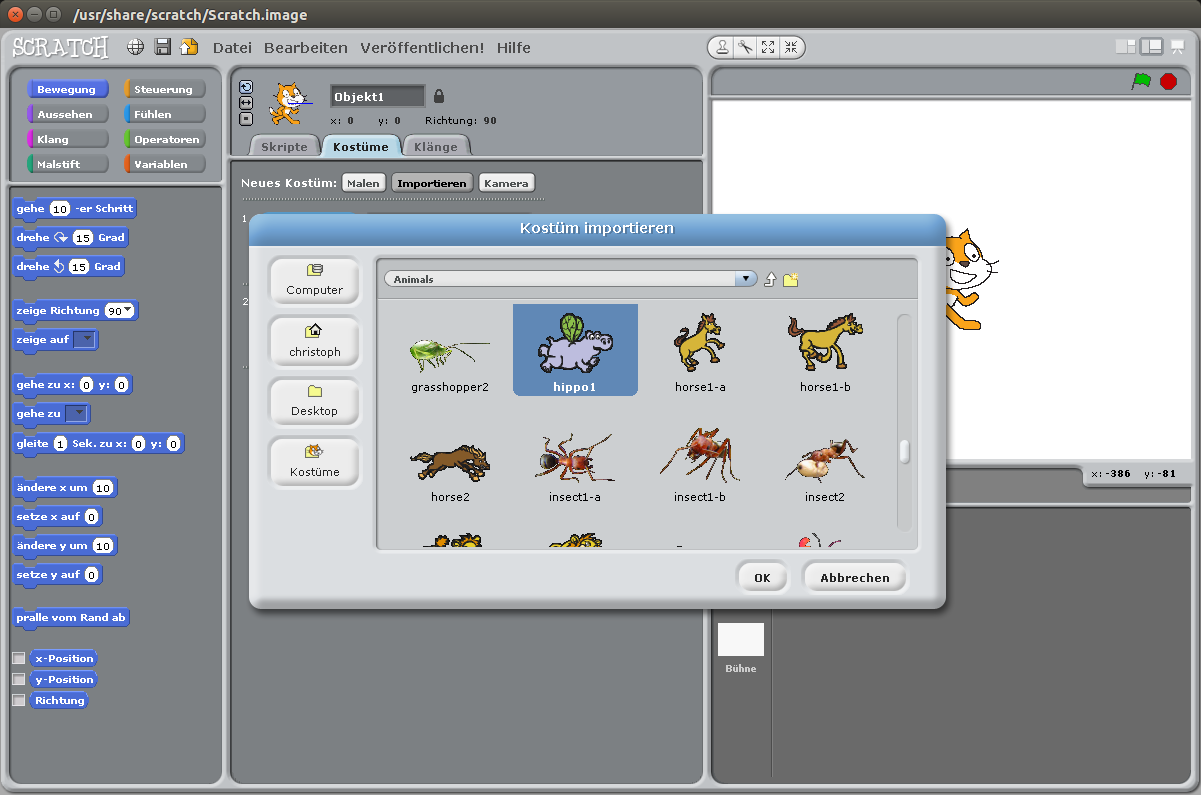
\includegraphics[width=\textwidth]{images/aufgabe1_tiere.png}

\subsubsection{Bewege deinen Sprite in 4 Richtungen (Rechts, Links, Hoch, Runter)}

Sprites können eigentlich nichts von sich aus. Eine Sprite-Aktion kommt direkt aus einem Skript aus dem Skript-Editor. Diese Skripte sind die Anweisungen für genau das was ein Sprite tun soll.
Du ziehst die Anweisung mit deiner Maus aus der linken Kachelspalte in die Skriptspalte. Die Kacheln passen wie Puzzleteile ineinander und bilden eine Anweisung.


\begin{itemize}
\item[1.] Klicke auf den Sprite-Reiter
\item[2.] Wenn du dein Sprite nach rechts bewegen willst, klicke auf den Steuerung-Button.
\end{itemize}
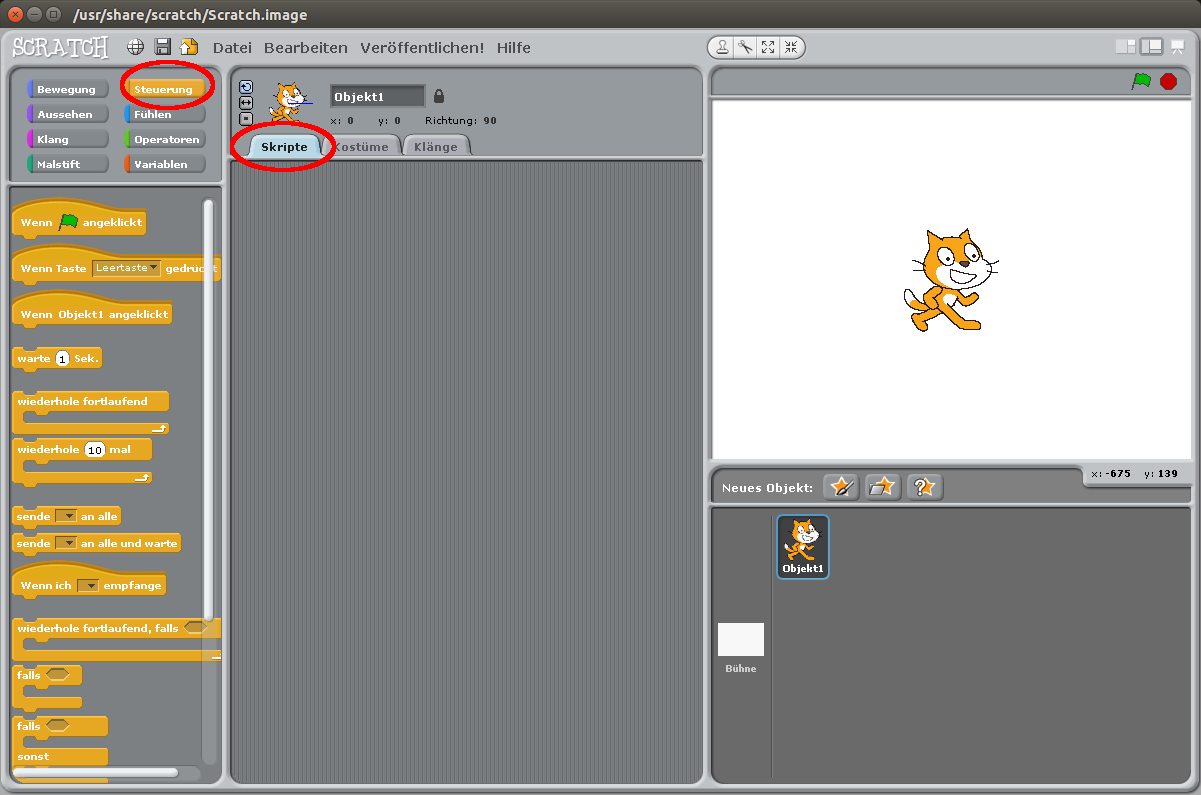
\includegraphics[width=\textwidth]{images/aufgabe1_steuerung.png}

\begin{itemize}
\item[3.] Klicke mit der linken Maustaste auf eine Anweisung und halte die Taste gedrückt. Ziehe nun den Befehl
 \textit{Wenn Taste Leertaste gedrückt} nach rechts in die Skriptfläche. 
\end{itemize}
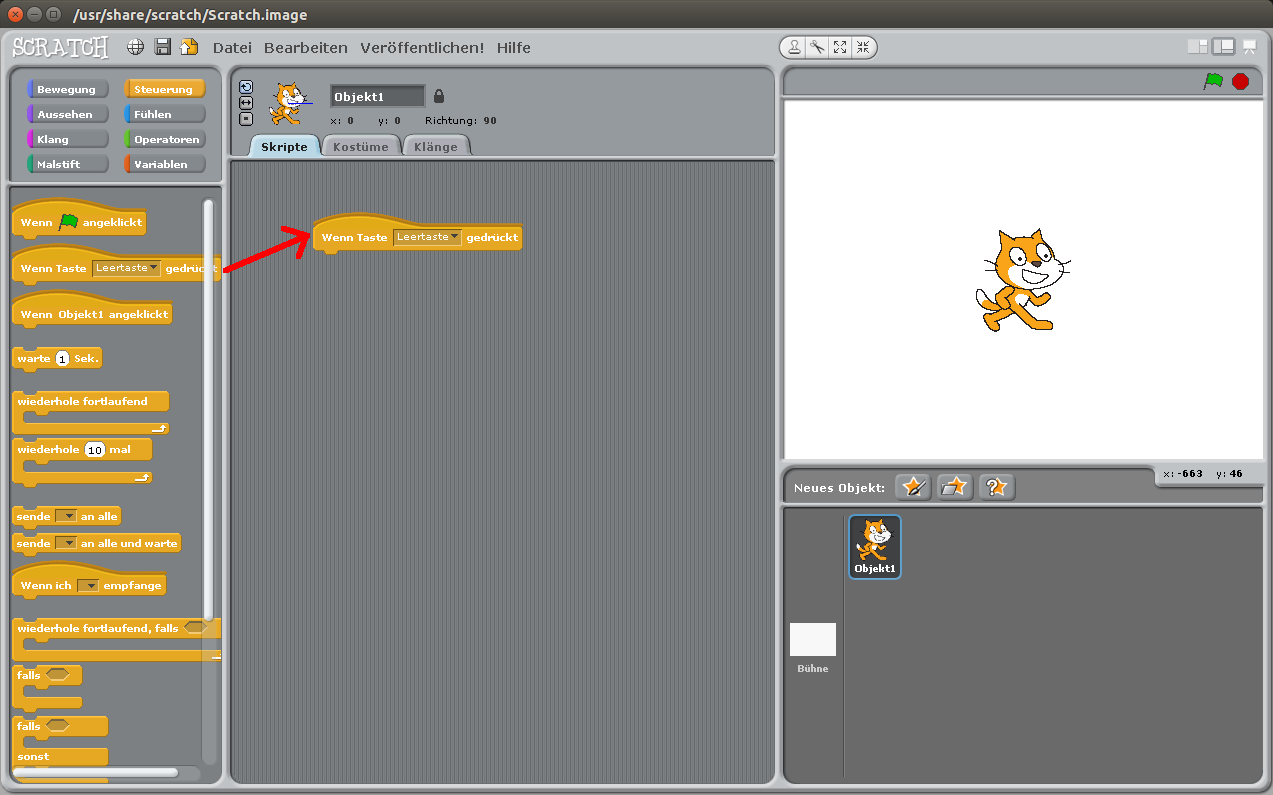
\includegraphics[width=\textwidth]{images/aufgabe1_steuerung_verschieben.png}

\begin{itemize}
\item[4.] Klicke auf das Wort \textit{Leertaste} und wähle \textit{Pfeil nach rechts} aus.  (Wir bewegen den Sprite nach rechts)
\end{itemize}
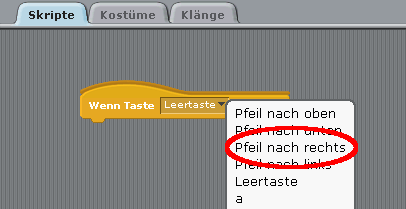
\includegraphics[width=0.5\textwidth]{images/aufgabe1_dropdown.png}

\begin{itemize}
\item[5.] Klicke auf den Bewegung-Button, oben links, und ziehe die Kachel “zeige Richtung 90” in das Skript-Fenster.
\end{itemize}
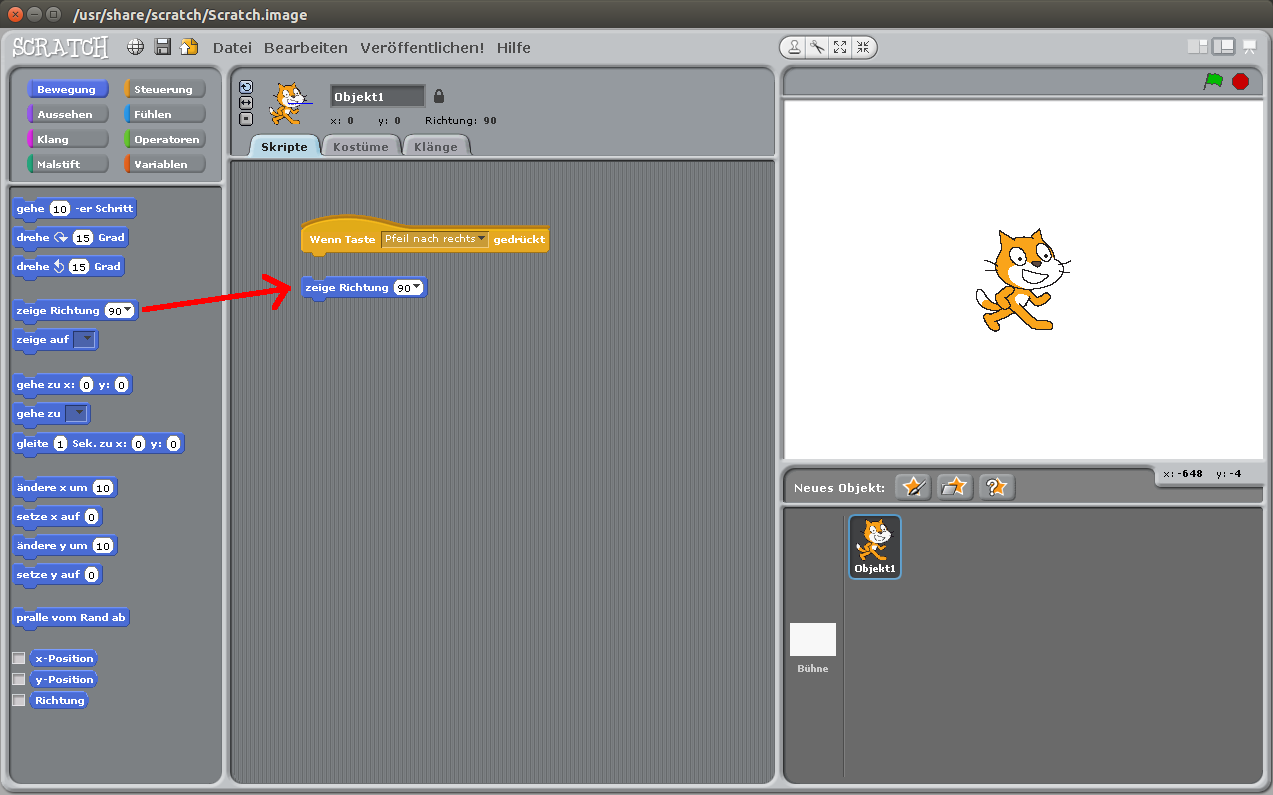
\includegraphics[width=\textwidth]{images/aufgabe1_bewegung_verschieben.png}

\begin{itemize}
\item[6.] Verbinde \textit{Wenn Taste Pfeil nach Rechts} mit \textit{zeige Richtung 90}
\item[7.] Klicke auf das \textit{gehe 10-er Schritte} und ziehe es in das Skript-Fenster 
\item[8.] Verbinde die Kacheln wie auf dem Bild. 
\end{itemize}
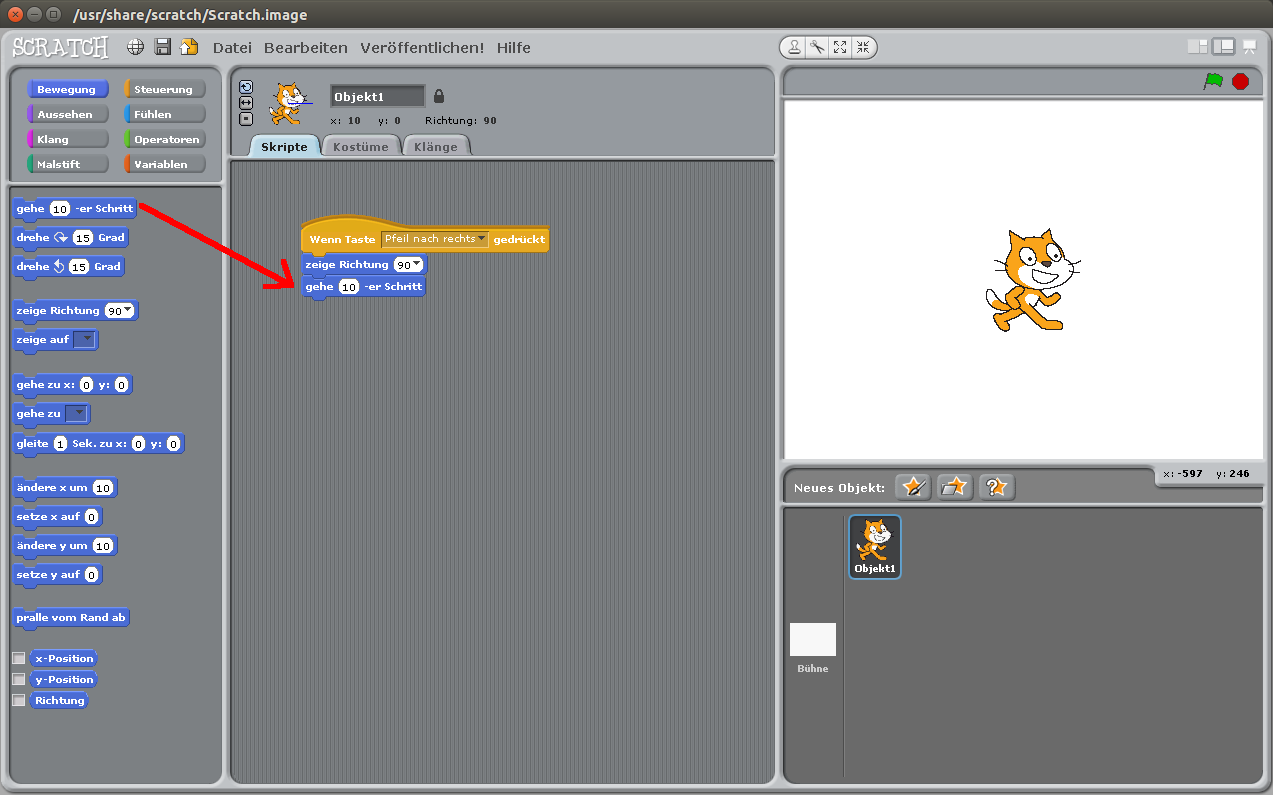
\includegraphics[width=\textwidth]{images/aufgabe1_bewegung_verschieben2.png}

\begin{itemize}
\item[9.] Klicke den Pfeil-Button deiner Tastatur und deine Figur bewegt sich.
\end{itemize}

Baue nun die gleiche Steuerung für die anderen drei Richtungen!

\begin{itemize}

\item[10.] Bewegen wir unser Sprite nach links: Drag Ziehe den \textit{wenn Leertaste gedrückt}-Button in das Skriptfenster .
\item[11.] Ändere \textit{Leertaste} zu \textit{Pfeil nach links gedrückt}
\item[12.] Ziehe \textit{zeige Richtung 90} aus dem Bewegungsfenster in das Skript-Fenster.
\item[13.] Ändere die 90 zu -90.
\item[14.] Ziehe die \textit{gehe 10er Schritte}-Kachel in das Skriptfenster und verbinde es mit der vorherigen Kachel.
( Wenn es bei dir aussieht wie auf dem Bild, ist alles korrekt!)
\end{itemize}
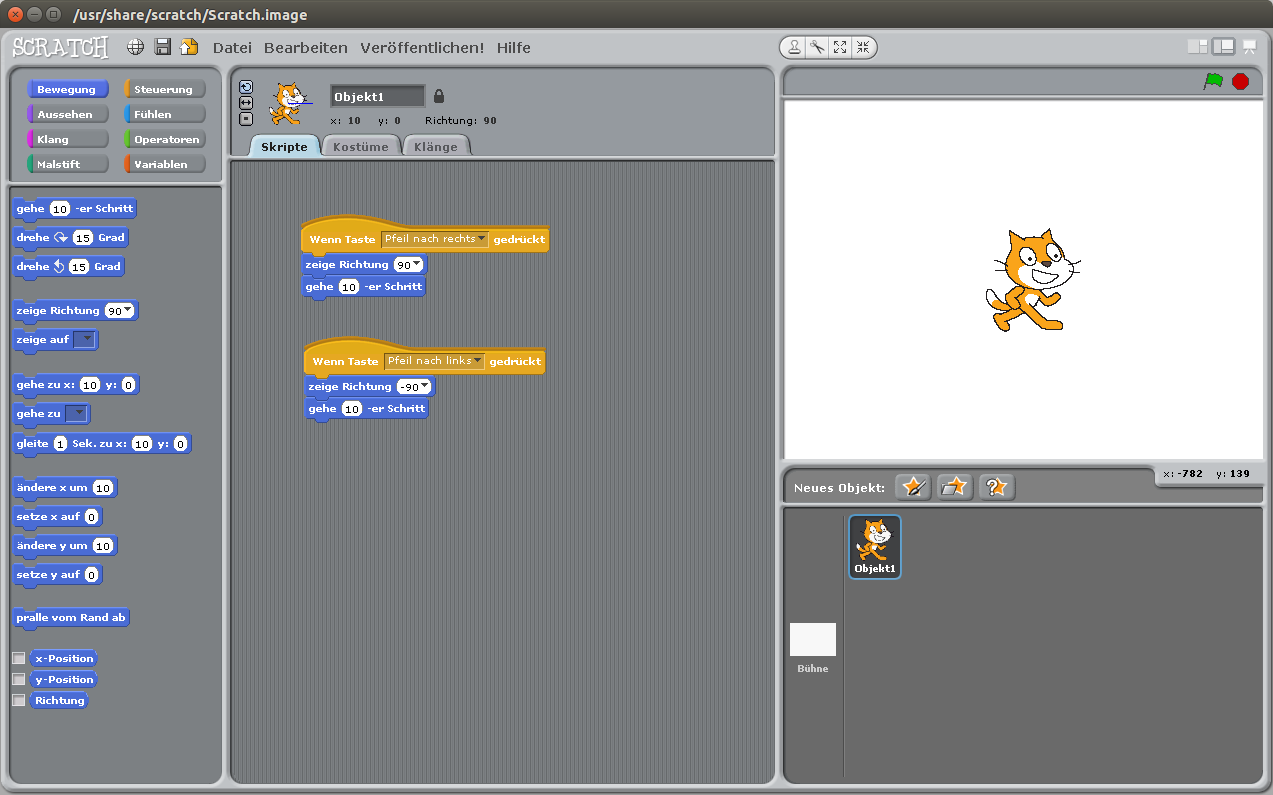
\includegraphics[width=\textwidth]{images/aufgabe1_links.png}

\begin{itemize}
\item[15.] Jetzt sollte auch dein linker Pfeil auf der Tastatur funktionieren! Klicke auf den Doppelpfeil, damit sich die Figur auch in die richtige Laufrichtung dreht. 
\item[16.] Lass deine Figur sich nach unten bewegen: Ziehe und verbinde dazu folgende Kacheln:
\subitem \textit{Wenn Leertaste gedrückt}
\subitem \textit{Zeige Richtung 90}
\subitem \textit{gehe 10 Schritte}
\item[17.] Ändere \textit{Leertaste} zu \textit{Pfeil nach unten}
\item[18.] Jetzt funktioniert auch der Pfeil nach unten auf deiner Tastatur. 
\end{itemize}
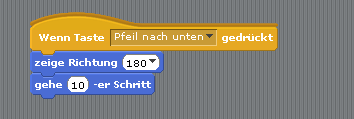
\includegraphics[width=0.6\textwidth]{images/aufgabe1_unten.png}

\begin{itemize}
\item[19.] Lass deine Figur sich nach oben bewegen: Ziehe und verbinde dazu folgende Kacheln:
\subitem \textit{Wenn Leertaste gedrückt}
\subitem \textit{Zeige Richtung 90}
\subitem \textit{gehe 10 Schritte}
\item[20.] Setze die Richtung auf  \textit{0 - Oben}:
\item[21.] Ändere \textit{Leertaste} zu \textit{Pfeil nach oben}
\end{itemize}
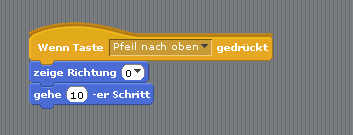
\includegraphics[width=0.6\textwidth]{images/aufgabe1_oben.png}

\begin{itemize}
\item[22.] Jetzt bewegt sich dein Sprite in alle 4 Richtungen. Überprüfe es !
\end{itemize}
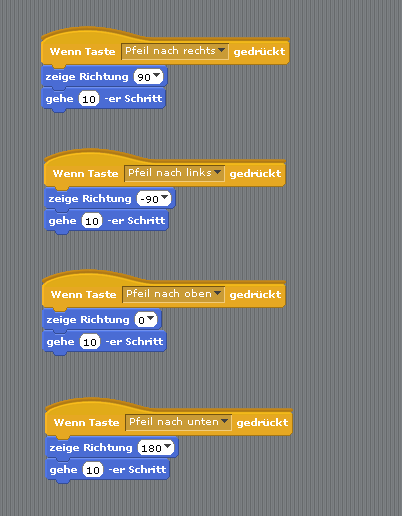
\includegraphics[width=0.6\textwidth]{images/aufgabe1_vier_richtungen.png}

\begin{itemize}
\item[23.] Gib deinem Sprite einen Namen.
\end{itemize}
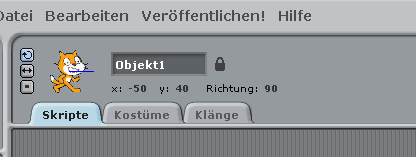
\includegraphics[width=0.6\textwidth]{images/aufgabe1_name_aendern_alt.png} \newline
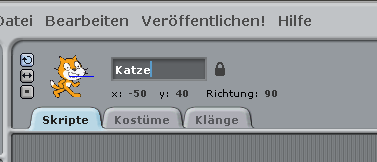
\includegraphics[width=0.6\textwidth]{images/aufgabe1_name_aendern.png}
\begin{itemize}
\newpage
\item[24.] Speichere dein Programm
\end{itemize}
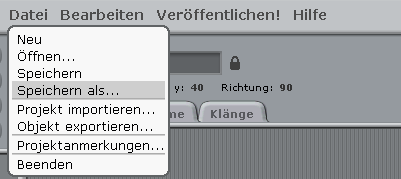
\includegraphics[width=0.6\textwidth]{images/aufgabe1_name_speichern1.png} \newline
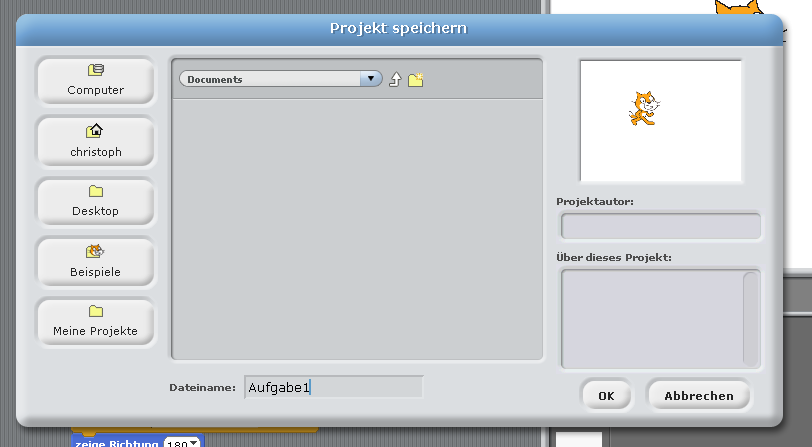
\includegraphics[width=0.6\textwidth]{images/aufgabe1_name_speichern2.png}